\begin{figure}[!htb]
\centering
\caption{Growth of \$1 invested on \res{first_decision} (log scale), net of costs unless stated. The dashed line shows the
strategy before trading costs.}\label{fig:cumulative}
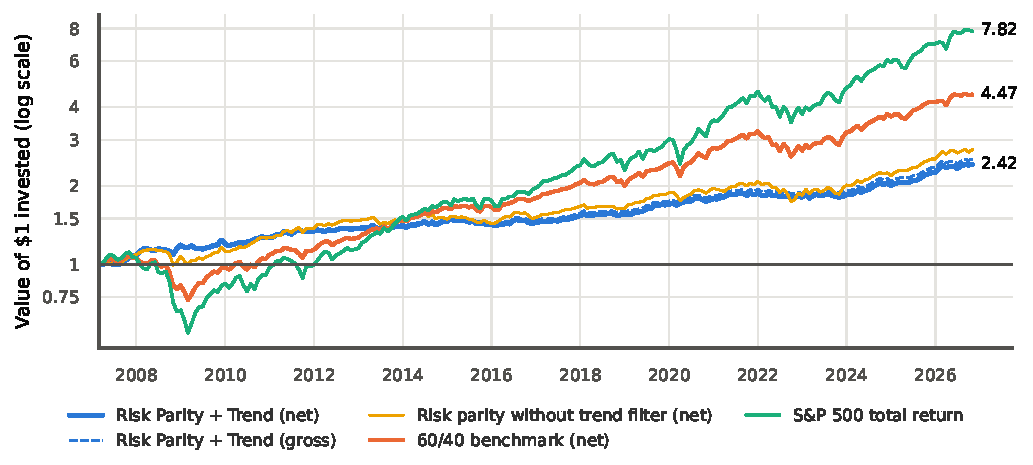
\includegraphics[width=\textwidth]{figures/fig_cumulative.pdf}\resmark{fig_cumulative}
\end{figure}

Figure~\ref{fig:cumulative} shows the central trade-off: \$1 grew to \$\res{strat_final_value} in the strategy,
\$\res{b6040_final_value} in 60/40 and \$\res{mkt_final_value} in the S\&P 500. The strategy led until 2014 because it avoided
the 2008 crash, then fell behind in the long bull market. Table~\ref{tab:performance} reports all measures.

\begin{table}[!htb]
\centering\small
\caption{Performance \res{sample_start}--\res{sample_end}, monthly returns, net of \res{cost_bps} per unit of turnover
(except ``Gross'')}\label{tab:performance}
\begin{threeparttable}
\begin{tabular}{@{}lrrrrrr@{}}
\toprule
\rowcolor{fmdark}\textcolor{white}{\textbf{Mar 2007--Oct 2026}} & \textcolor{white}{\textbf{Strategy}} & \textcolor{white}{\textbf{Gross}} & \textcolor{white}{\textbf{ERC}} & \textcolor{white}{\textbf{1/N}} & \textcolor{white}{\textbf{60/40}} & \textcolor{white}{\textbf{S\&P 500}} \\
\rowcolor{fmlight}\multicolumn{7}{@{}l}{\textbf{Return and risk}} \\
Average return (\% p.a.) & 4.6 & 4.8 & 5.4 & 7.1 & 8.1 & 11.7 \\
CAGR (\% p.a.) & 4.6 & 4.8 & 5.3 & 6.7 & 7.9 & 11.0 \\
Volatility (\% p.a.) & 4.7 & 4.7 & 7.1 & 11.3 & 9.9 & 15.4 \\
Sharpe ratio & 0.66 & 0.71 & 0.55 & 0.50 & 0.67 & 0.66 \\
Maximum drawdown (\%) & $-$5.7 & $-$5.4 & $-$16.0 & $-$36.8 & $-$32.3 & $-$50.9 \\
Worst 12 months (\%) & $-$5.7 & $-$5.4 & $-$13.4 & $-$34.2 & $-$27.7 & $-$43.3 \\
\rowcolor{fmlight}\multicolumn{7}{@{}l}{\textbf{Relative to the market (S\&P 500 TR)}} \\
Beta & 0.10 & 0.10 & 0.29 & 0.61 & 0.63 & 1.00 \\
Alpha (\% p.a.) & 2.1 & 2.3 & 0.9 & $-$0.6 & 0.2 & $-$0.0 \\
\quad $t$-stat (Newey-West) & 2.10 & 2.34 & 0.68 & $-$0.37 & 0.43 & -- \\
\rowcolor{fmlight}\multicolumn{7}{@{}l}{\textbf{Relative to the 60/40 benchmark}} \\
Beta & 0.19 & 0.19 & 0.53 & 0.98 & -- & 1.54 \\
Alpha (\% p.a.) & 1.8 & 2.0 & 0.4 & $-$0.9 & -- & 0.0 \\
\quad $t$-stat (Newey-West) & 1.90 & 2.14 & 0.35 & $-$0.58 & -- & 0.04 \\
Tracking error (\% p.a.) & 9.0 & 9.0 & 6.7 & 5.8 & -- & 6.0 \\
Information ratio & $-$0.39 & $-$0.36 & $-$0.41 & $-$0.18 & -- & 0.59 \\
\rowcolor{fmlight}\multicolumn{7}{@{}l}{\textbf{Implementation}} \\
Turnover (\% p.a.) & 215.7 & 215.7 & 51.1 & 37.5 & 24.4 & -- \\
Average T-bill weight (\%) & 31.6 & 31.6 & 0.0 & 0.0 & 0.0 & -- \\
Final value of \$1 & 2.42 & 2.52 & 2.75 & 3.55 & 4.47 & 7.82 \\
\bottomrule
\end{tabular}
\resmark{tab_performance}
\begin{tablenotes}\footnotesize
\item ERC = risk parity without trend filter; 1/N = equal weights without trend filter. Average return arithmetic $\times 12$;
volatility $\times\sqrt{12}$; Sharpe ratio on excess returns over T-bills; beta not annualised; alpha $\times 12$ (Jensen's
alpha); information ratio = annualised active return / tracking error. Turnover includes the initial purchase.
\end{tablenotes}
\end{threeparttable}
\end{table}

\textbf{What the measures mean for our client.}
\begin{itemize}[leftmargin=1em]
\item \emph{Average return} \res{strat_ann_mean} p.a. vs \res{b6040_ann_mean}: the client gives up about half of the 60/40
return, but still grows well above the T-bill rate of \res{rf_mean}.
\item \emph{Volatility} \res{strat_ann_vol} vs \res{b6040_ann_vol}: swings are about \res{vol_ratio_6040} times those of 60/40,
the risk of a short-to-medium bond fund rather than a balanced fund.
\item \emph{Sharpe ratio} \res{strat_sharpe} vs \res{b6040_sharpe}: the same reward per unit of risk; not a better portfolio, but a
\emph{less risky} one. With a standard error of about \res{sharpe_se} \citep{lo2002} the two are statistically indistinguishable.
\item \emph{Beta} \res{strat_beta_mkt} against the S\&P 500 (\res{strat_beta_bench} against 60/40): a 10\% equity fall implies a
loss of only about \res{beta_mkt_loss10}\%. The return hardly depends on the stock market.
\item \emph{Alpha} \res{strat_alpha_mkt} p.a. against the market ($t=\res{strat_alpha_mkt_t}$) and \res{strat_alpha_bench} against
60/40 ($t=\res{strat_alpha_bench_t}$): more than the CAPM predicts given the low market exposure. It is borderline significant
and mainly reflects Treasuries, gold and commodities, which a stock-market factor misses.
\item \emph{Information ratio} \res{strat_info_ratio} against 60/40, tracking error \res{strat_tracking_error}: the strategy
underperformed 60/40 and deviated from it a lot. Clients who judge success against 60/40 should not buy it; for our client
the drawdown matters.
\item \emph{Maximum drawdown} \res{strat_max_dd} vs \res{b6040_max_dd} (S\&P 500: \res{mkt_max_dd}): about a sixth of the 60/40
loss. Worst 12 months: \res{strat_worst_12m} vs \res{b6040_worst_12m}.
\item \emph{At equal risk:} levered monthly to a volatility target near that of 60/40 (realised \res{ext_lev10_ann_vol}; borrowing
slightly above the T-bill rate, before taxes), the strategy would have earned \res{ext_lev10_cagr} a year vs \res{b6040_cagr},
with a maximum drawdown of \res{ext_lev10_max_dd} vs \res{b6040_max_dd}. Capped at two times leverage, more realistic for private
clients, and borrowing at T-bills + 10 bps: \res{imp_lev_cap2_s10_cagr} a year (Sharpe ratio \res{imp_lev_cap2_s10_sharpe},
maximum drawdown \res{imp_lev_cap2_s10_maxdd}).
\end{itemize}

\begin{figure}[!htb]
\centering
\caption{Drawdown from the previous peak, net of costs.}\label{fig:drawdowns}
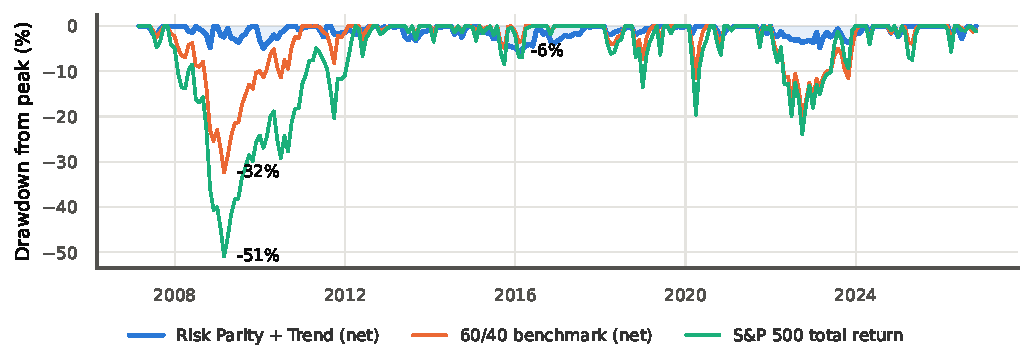
\includegraphics[width=\textwidth]{figures/fig_drawdowns.pdf}\resmark{fig_drawdowns}
\end{figure}

\textbf{Stress periods.} Financial crisis (Nov 2007--Feb 2009): strategy \res{strat_gfc}, 60/40 \res{b6040_gfc}; Covid crash
(Feb--Mar 2020): \res{strat_covid} vs \res{b6040_covid}; 2022 rate shock (Jan--Oct 2022): \res{strat_infl} vs \res{b6040_infl},
because the filter also sold Treasuries. The price is paid in recoveries: 2023--Oct 2026 \res{strat_recov} vs \res{b6040_recov}.
Figure~\ref{fig:weights} shows the shift into T-bills in falling markets.

\begin{figure}[!htb]
\centering
\caption{Target weights at each monthly rebalancing date. Grey: T-bills held because an asset class is below trend.}\label{fig:weights}
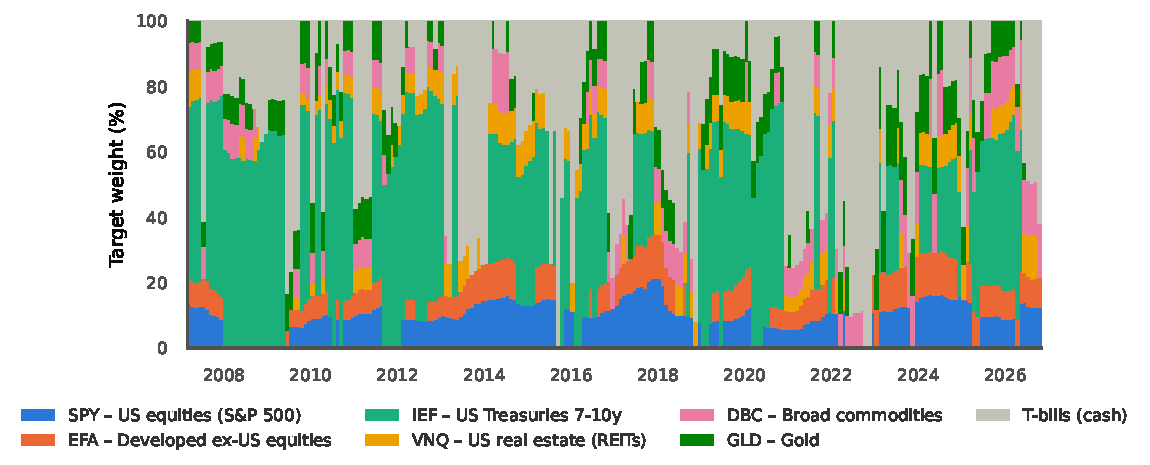
\includegraphics[width=\textwidth]{figures/fig_weights.pdf}\resmark{fig_weights}
\end{figure}
